\documentclass{standalone}
\usepackage{tikz}

\begin{document}

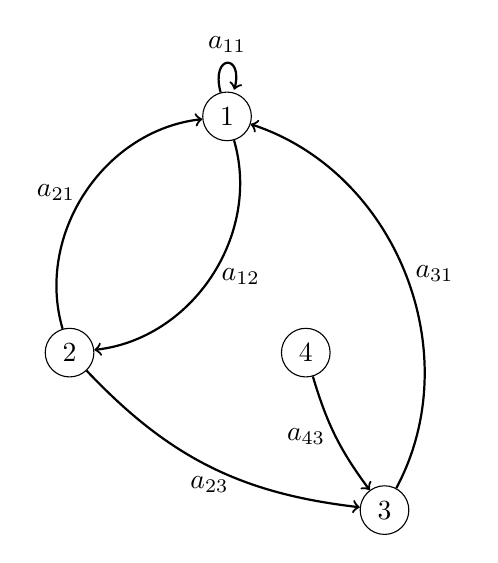
\begin{tikzpicture}
  \node[circle, draw] (1) at (-1, 3) {1};
  \node[circle, draw] (2) at (-3, 0) {2};
  \node[circle, draw] (3) at (1, -2) {3};
  \node[circle, draw] (4) at (0, 0) {4};
  \draw[->, thick, black]
  (1) edge [bend left=50, right] node {$a_{12}$} (2)
  (2) edge [bend left=50, left] node {$a_{21}$} (1)
  (2) edge [bend right=20, below] node {$a_{23}$} (3)
  (3) edge [bend right=50, right] node {$a_{31}$} (1)
  (4) edge [bend right=10, left] node {$a_{43}$} (3)
  (1) edge [loop above] node {$a_{11}$} (1);
\end{tikzpicture}
 
\end{document}
